\documentclass[a4paper]{article}
\usepackage{latexsym}
\usepackage[a4paper]{geometry}
\usepackage{color}
\usepackage{listings}
\usepackage[pdftex]{graphicx}
\usepackage{subfig}
\usepackage{float}

\definecolor{Blue}{rgb}{0,0,0.5}
\definecolor{Green}{rgb}{0,0.75,0.0}
\definecolor{LightGray}{rgb}{0.6,0.6,0.6}
\definecolor{DarkGray}{rgb}{0.3,0.3,0.3}
\lstset{language=Matlab,
   keywords={function,uint8,uint16,uint32,double,break,case,catch,continue,else,elseif,end,for,global,if,otherwise,persistent,return,switch,try,while},
   basicstyle=\ttfamily\small,
   breaklines=true,
   keywordstyle=\bfseries\color{Blue},
   commentstyle=\itshape\color{LightGray},
   stringstyle=\color{Green},
   numbers=left,
   numberstyle=\tiny\color{DarkGray},
   stepnumber=1,
   numbersep=10pt,
   backgroundcolor=\color{white},
   tabsize=2,
   showspaces=false,
   showstringspaces=false,
   captionpos=b}

%Boldface text for type writer font
\usepackage{bold-extra} %\DeclareFontShape{OT1}{cmtt}{bx}{n}{<5><6><7><8><9><10><10.95><12><14.4><17.28><20.74><24.88>cmttb10}{}

%Break words properly at the end of a line (which isn't sloppy...)
\sloppy

%Use command \exercise for each exercise
\newcounter{exerciseCount}
\setcounter{exerciseCount}{0}
\newcommand{\exercise}[1]{\addtocounter{exerciseCount}{1} \noindent \medskip {\large \textsf{\textbf{Exercise \arabic{exerciseCount} \--- #1}}} \par}
\renewcommand{\theenumi}{\textsf{\textbf{\alph{enumi}}}}

%Use command \code for code snippets
\newcommand{\code}[1]{\textnormal{\texttt{#1}}}



\title{\textsf{Image Processing \\ lab 3}}
\author{Klaas Kliffen \and Jan Kramer}
\date{\today}

\begin{document}
\maketitle

\exercise{1-D wavelet transforms}
\begin{enumerate}
\item

%Assuming the length of the input vector is a power of two,
%it is possible to iterate over the input vector applying the algoritm described by example 7.8.
%The current length is initialized to the length of the vector. For each step, this length is halved.
%Since the input vector of a step is split in half, a part with sums and a part with differences,
%the next step will only use the sums, as specified by the algoritm.
%First two vector are created by taking the odd and even element of the input vector until the current length of the scale.
%Two result vectors are calculated for the sums and the differences.
%The difference vector is positioned after the sum vector and written to the input vector.
%The values of the sum and difference vector needs normalization, which is a factor of the square root of 2.
The algorithm given in the assignment can be represented as a filter bank based on the Haar scaling and wavelet vectors.
Normally the whole input would be convolved with these vectors.
However since the two-point sums and differences are taken, this convolution is combined with downscaling.
Our implementation of a $j$-scale DWT is based on this algorithm by applying this ``filter bank'' $j$ times.
Otherwise its implementation is rather trivial.

\lstinputlisting{../lab3ex1/IPdwt.m}
\item 
The inverse of the wavelet transform is basicly doing all steps from the \lstinline|IPdwt| in reverse.
The inital length is set to the end of the length of the last sum vector.
This can be determined by taking the lenght and divide it by a power of 2 with the scale.
Then for each step the sum and difference vectors are retrieved from the input vector by taking halves of the input vector.
Two new component vectors are created for the values. These need to be scaled again to retrieve the right results.
The component vectors are then interleaved and replace their original values in the input vector.
This is repeated until the orignal scale of the transformation is reached.
\lstinputlisting{../lab3ex1/IPidwt.m}
\end{enumerate}


\exercise{2-D wavelet transforms}
\begin{enumerate}
\item
According to the Section $7.5$ in the book the extension of 1D DWT to 2D is simple, because of the separable scaling and wavelet functions.
It also mentions that the 2D DWT can be computed by first doing a 1D DWT of the columns and then doing a 1D DWT of the rows.
Note that one could also calculate the DWT first for rows and then for columns.
Our implementation uses this fact.
In each iteration $j$ the algorithm of exercise 1 is applied to each row and then to each column to get the approximation, the horizontal detail, the vertical detail and the diagonal detail.

\lstinputlisting{../lab3ex2/IPdwt2.m}
\item
The result of the IPdwt2 by itself is too dark to see details clearly, since the values in the detail parts of the resulting image are around zero(black).
Therefore our implementation shifts the input image to the 2d DWT such that the resulting details are centered around a gray value.
After that we can constrast-stretch the various detail images by iterating over the $j$-scale and at the end the approximation image is stretched.

\lstinputlisting{../lab3ex2/IPdwt2scale.m}
\item
In Figure~\ref{fig:wavelet} the images with labels 1, 4 and 7 are horizontal details of scale 1, 2 and 3 respectivily.
Similarly images with labels 2, 5 and 8 are diagonal details with scale 1, 2 and 3 respectivily.
In addition images with labels 3, 6 and 9 are vertical details with scale 1, 2 and 3 respectivily.
And at last the image with label 10 is the approximation image of scale 3.
\begin{figure}[H]
\centering
\begin{tabular}{ccc}
    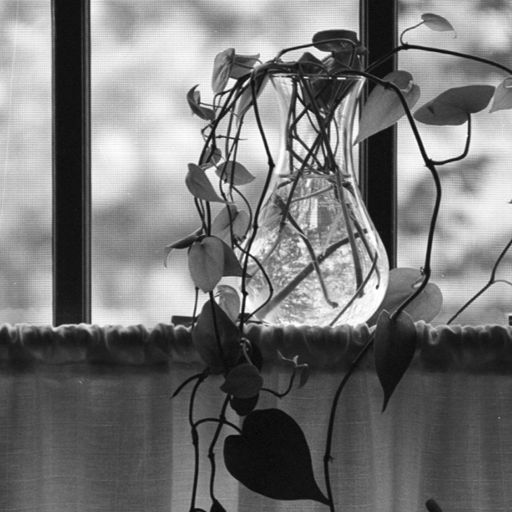
\includegraphics[width=0.3\textwidth]{../lab3ex2/vase.png} & 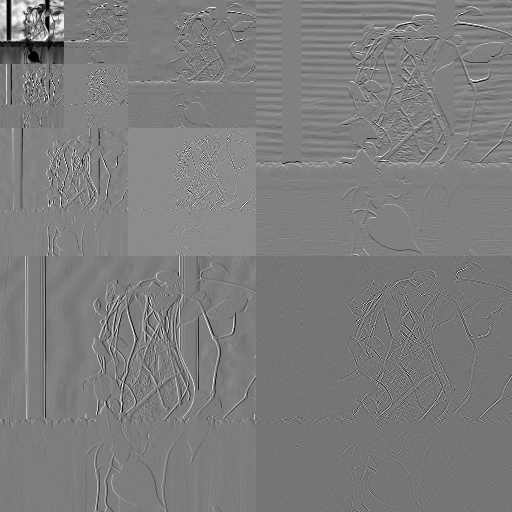
\includegraphics[width=0.3\textwidth]{../lab3ex2/scaled.png}  & 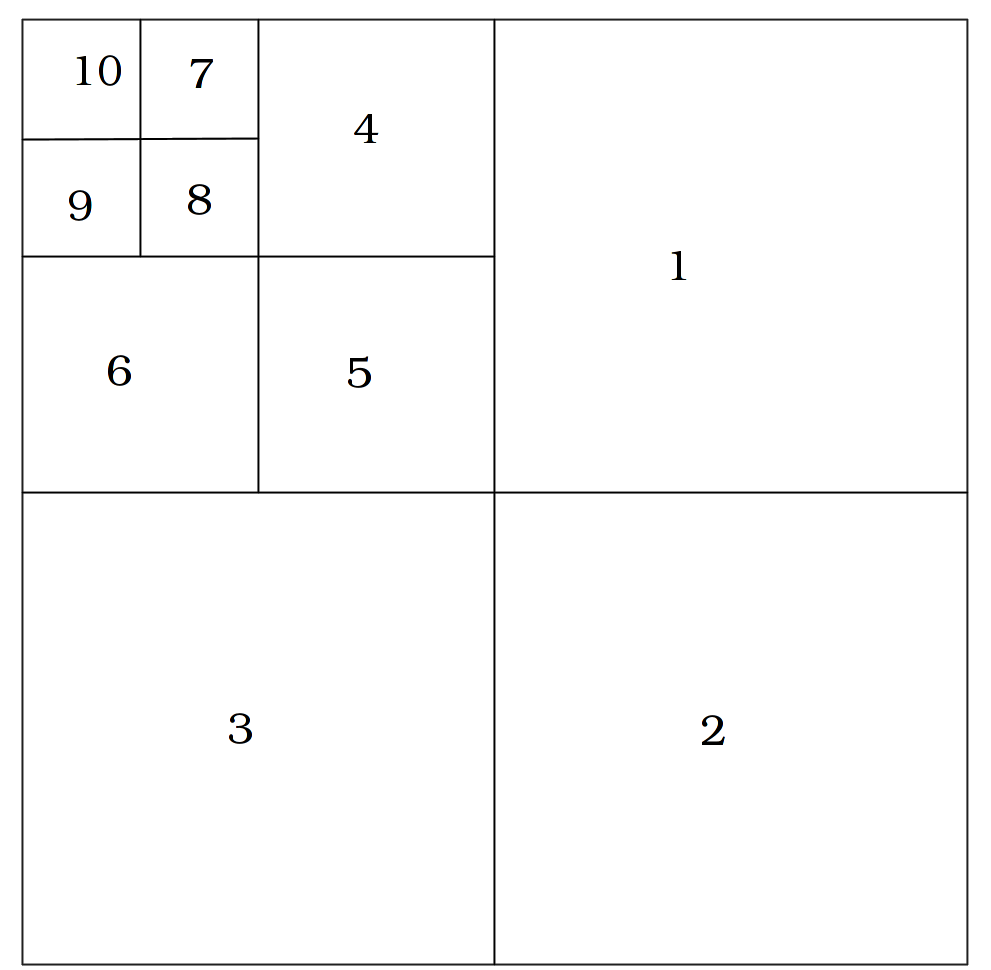
\includegraphics[width=0.3\textwidth]{layout.png}\\
    Original image & 3 scale wavelet transform & the layout labels of the transform \\
\end{tabular}
\caption{3 scale wavelet transform of the orignal image}
\label{fig:wavelet}
\end{figure}

\item
According to Section $7.5$ the 2D inverse DWT can also be computed by using a 1D inverse DWT function.
So similarly on how our 2D DWT implementation is based on our 1D DWT implemention, the 2D inverse DWT is also based on the 1D DWT implementation.
Note however that the order of applying 1D DWT first to rows and then columns in the 2D DWT, has to be inverted in the 2D inverse DWT.
Hence our iplementation first applies a 1D inverse DWT to the columns and the one to the rows.
\lstinputlisting{../lab3ex2/IPidwt2.m}
\begin{figure}[H]
\centering
\begin{tabular}{cc}
 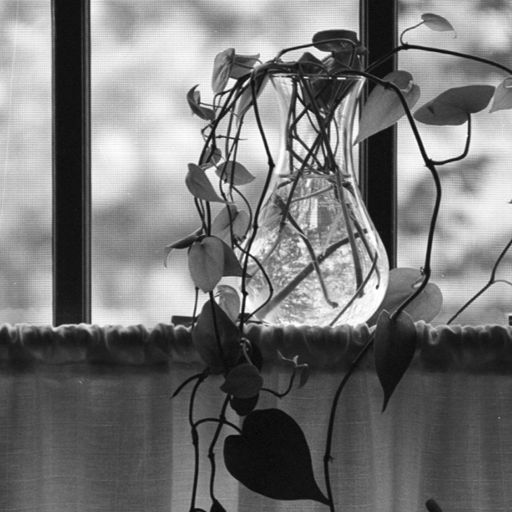
\includegraphics[width=0.4\textwidth]{../lab3ex2/vase.png} & 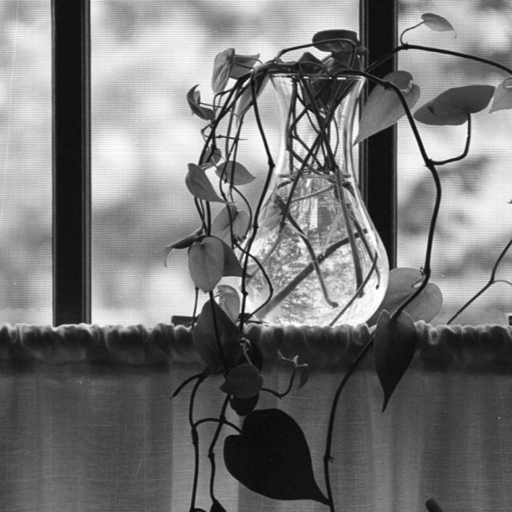
\includegraphics[width=0.4\textwidth]{../lab3ex2/output.png} \\
 Original image & Restoration of the image form figure \ref{fig:wavelet} \\
\end{tabular}
\caption{3 scale wavelet transform restoration}
\label{fig:waveletback}
\end{figure}

\end{enumerate}

\exercise{Image Compression}
\begin{enumerate}
\item
First the wavelet transform is performed on the input image.
A threshold matrix consisting solely of the threshold value is used to find all pixels larger than the threshold in the transform.
The thresholded image is then retrieved by pointwise multiplication of the results of comparing the threshold matrix with the wavelet transform.
Since the approximation of the original matrix is also passed by the threshold, it needs to be reconstructed.
This is done by copying the values from the wavelet transform back to the thresholded image.
The compressed image is then retrieved by applying the inverse wavelet transform.

\noindent The root mean square error and the mean square signal to noise ratio are calculated from the given formulas.
For the compression ratio the the build-in function of entropy is used to calculate the entropy of the compressed and
original image.
%TODO: Jan, klopt dit een beetje of is dit een beetje vaag/kort door de bocht.
The entropy is a value for how complex an image is and the minium amount of data which is needed to store the image.
Compressing the image lowers the complexity.
Dividing the original entropy by the compressed entropy yields a compression ratio.

\lstinputlisting{../lab3ex3/IPwaveletcompress.m}
\item
The quantitative properties for several different scales and thresholds can be seen in table \ref{tab:results}.
Globally the signal to noise ratio decreases and the errors and compression ratio increase while increasing scale and threshold.
Although for this image the increasing the scale past 9 was not possible, due to its size being a square of 512 pixels.
It would seem that increasing it further would not compress the image any further past a compression ratio of 37.
Increasing the threshold will yield in higher compression ratios. Although the signal to noise ratio decreases exponentiall, while
the errors increase almost linearly.
\begin{table}[H]
\centering
\begin{tabular}{r|r|r|r|r}
 \textbf{Scale} & \textbf{Threshold} & \textbf{$\epsilon_{rms}$} & \textbf{SNR} & \textbf{Compression ratio}\\
 \hline
 1 & 0.02 & 0.0086 & 1277.34 & 2.59:1 \\
 3 & 0.02 & 0.0157 &  385.47 & 17.42:1 \\
 3 & 0.05 & 0.0249 & 152.09  & 24.87:1 \\
 3 & 0.10 & 0.0322 & 90.33  & 29.14:1 \\
 5 & 0.02 & 0.0220 & 194.71  & 34.00:1 \\
 7 & 0.02 & 0.0272 & 127.44  & 36.40:1 \\
 7 & 0.05 & 0.0575 & 27.627  & 113.18:1 \\
 7 & 0.10 & 0.1035 & 7.837  & 460.20:1 \\
 9 & 0.02 & 0.0321 & 91.02   & 36.55:1 \\
\end{tabular}
\caption{Quantitative compression quality for different scales and threshold}
\label{tab:results}
\end{table}

\begin{figure}[H]
\centering
\begin{tabular}{cc}
 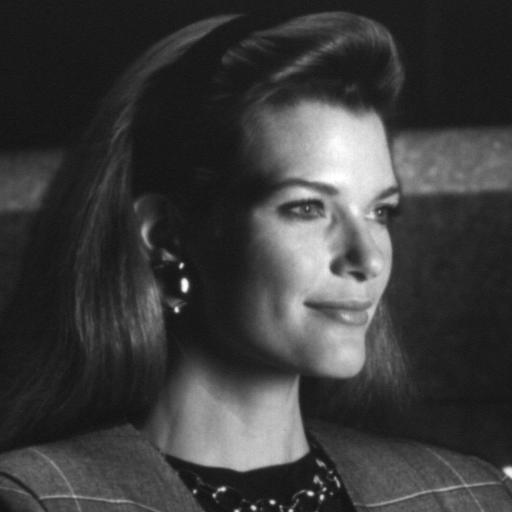
\includegraphics[width=0.4\textwidth]{../lab3ex3/tracy.png} & 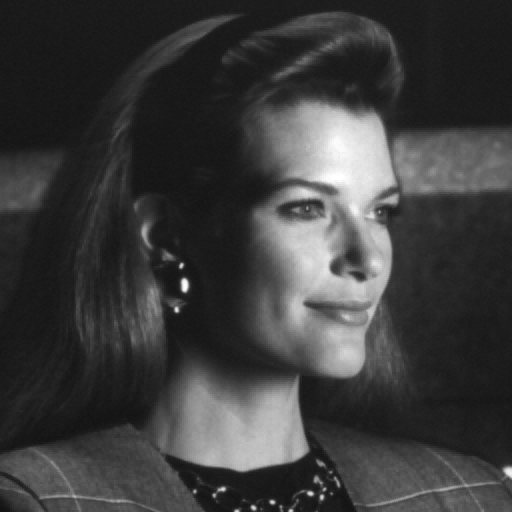
\includegraphics[width=0.4\textwidth]{../lab3ex3/l1t002.png} \\
 Original image & Scale: 1 Threshold: 0.02 \\
 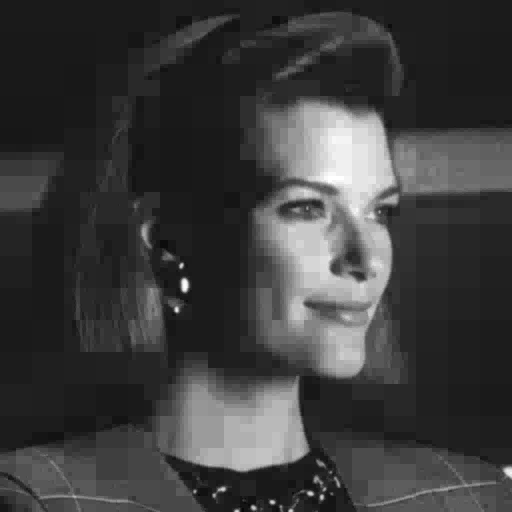
\includegraphics[width=0.4\textwidth]{../lab3ex3/l5t002.png} & 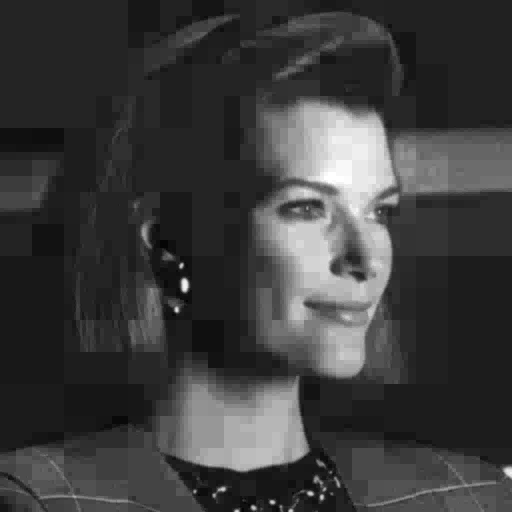
\includegraphics[width=0.4\textwidth]{../lab3ex3/l9t002.png}  \\
 Scale: 5 Threshold: 0.02 & Scale: 9 Threshold: 0.02 
\end{tabular}
\caption{Increasing wavelet compression scale on an image}
\label{fig:scaleinc}
\end{figure}

Figure \ref{fig:scaleinc} show the original image and the 3 compression with different scales.
Increasing the scale will cause square like artifacts of a single gray value.
The large spots are created because in with the high scale image, coarse details, such as the upper left corner become
small differences in the detail compents of that scale. 
The Thresholding will remove this detail, resulting in a monotone block.


\begin{figure}[H]
\centering
\begin{tabular}{cc}
 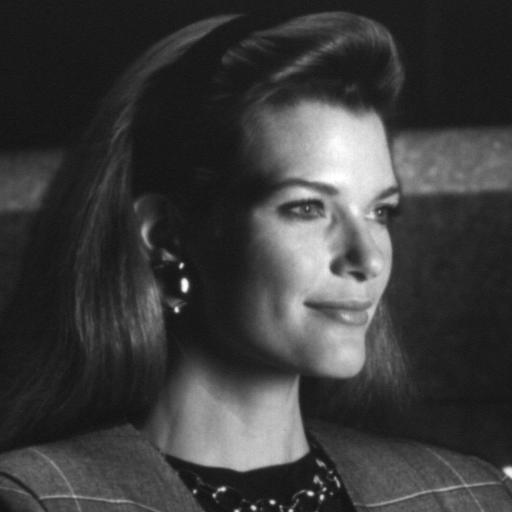
\includegraphics[width=0.4\textwidth]{../lab3ex3/tracy.png} & 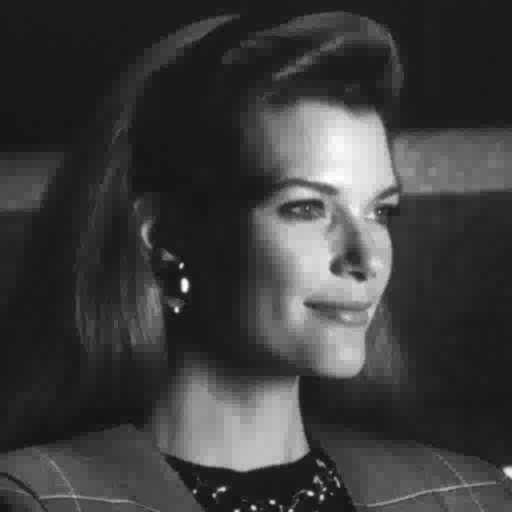
\includegraphics[width=0.4\textwidth]{../lab3ex3/l3t002.png} \\
 Original image & Scale: 3 Threshold: 0.02 \\
 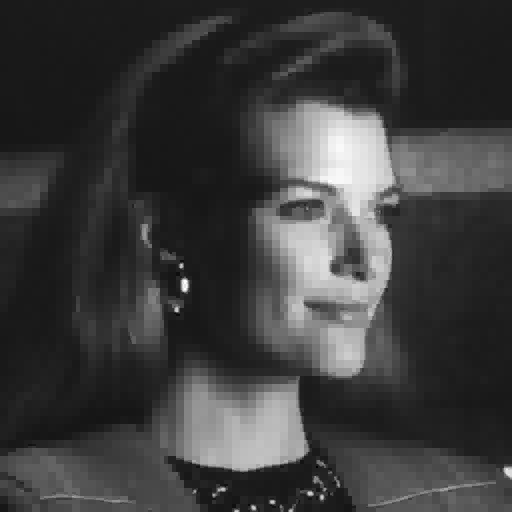
\includegraphics[width=0.4\textwidth]{../lab3ex3/l3t005.png} & 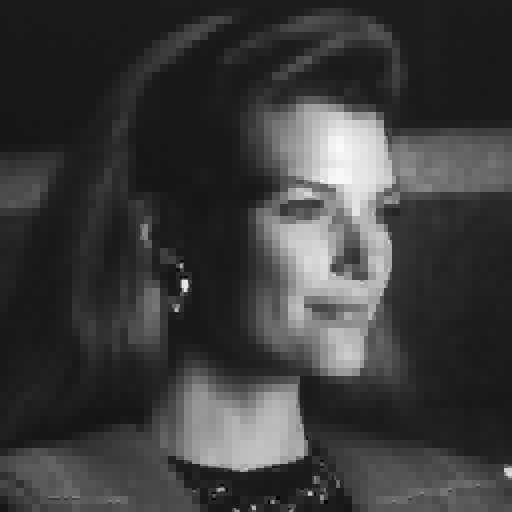
\includegraphics[width=0.4\textwidth]{../lab3ex3/l3t010.png}  \\
 Scale: 3 Threshold: 0.05 & Scale: 3 Threshold: 0.10 
\end{tabular}
\caption{Increasing wavelet compression threshold on scale 3 on an image}
\label{fig:scale3}
\end{figure}

Figure \ref{fig:scale3} show the compression on the orignal image with an increasing threshold.
The scale is quite low, so course details are not filtered. Increasing the threshold will remove the fine details.
This can be seen in a pixelated region around the face. This is caused by the lack of the detail component.
Essentially, the approximation image is just resized without increasing the detail, resulting in "large" pixels.

\begin{figure}[H]
\centering
\begin{tabular}{cc}
 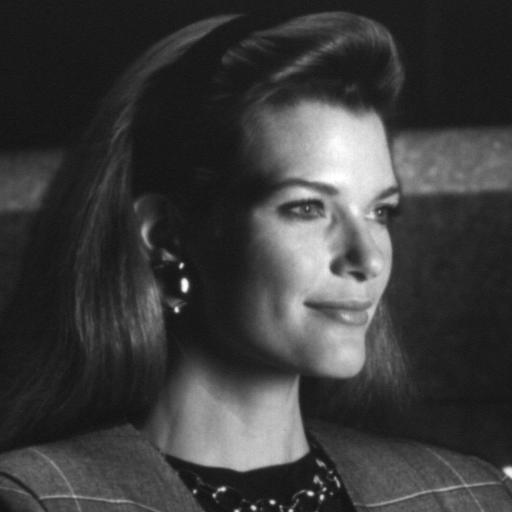
\includegraphics[width=0.4\textwidth]{../lab3ex3/tracy.png} & 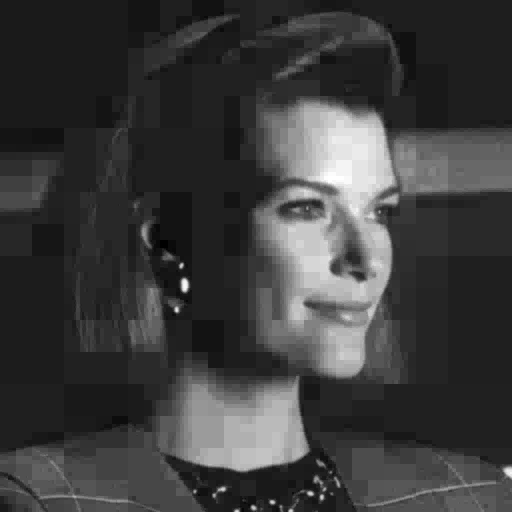
\includegraphics[width=0.4\textwidth]{../lab3ex3/l7t002.png} \\
 Original image & Scale: 7 Threshold: 0.02 \\
 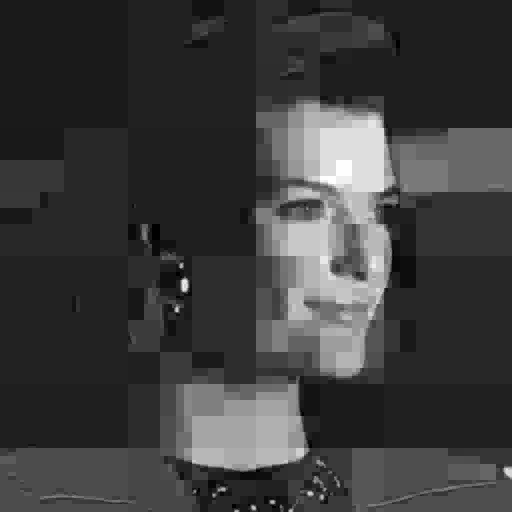
\includegraphics[width=0.4\textwidth]{../lab3ex3/l7t005.png} & 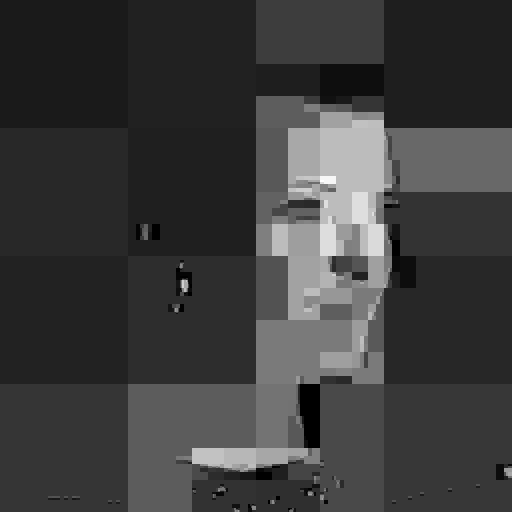
\includegraphics[width=0.4\textwidth]{../lab3ex3/l7t010.png}  \\
 Scale: 7 Threshold: 0.05 & Scale: 7 Threshold: 0.10 
\end{tabular}
\caption{Increasing wavelet compression threshold on scale 7 on an image}
\label{fig:scale7}
\end{figure}

Figure \ref{fig:scale7} shows the orignal image being compressed on a high scale with an increasing threshold.
The background is almost not visible anymore, only parts of the face contain a bit more detail.
This is caused by the higher scale. Course details on the higher scale do not have a large difference, thus are removed by the
threshold algorithm. This results in the large blocks in the lower right image.
The face contains still some detail, because this is detail is captured on a lower level and the amount of change is higher.
Thus a higher threshold is needed to remove that detail from the image.



\end{enumerate}

\newpage
\section*{Task distribution}

\begin{table}[H]
\centering
\begin{tabular}{ccccc}
ex1 & design & implementation & answers questions & writing report \\
\hline
Klaas & 60\% & 90\% & n.a. & 50\% \\
\hline
Jan & 40\% & 10\% & n.a. & 50\% \\
\end{tabular}
\end{table}

\begin{table}[H]
\centering
\begin{tabular}{ccccc}
ex2 & design & implementation & answers questions & writing report \\
\hline
Klaas & 50\% & 30\% & 25\% & 25\% \\
\hline
Jan & 50\% & 70\% & 75\% & 75\% \\
\end{tabular}
\end{table}

\begin{table}[H]
\centering
\begin{tabular}{ccccc}
ex3 & design & implementation & answers questions & writing report \\
\hline
Klaas & 50\% & 75\% & 50\% & 75\% \\
\hline
Jan & 50\% & 25\% & 50\% & 25\% \\
\end{tabular}
\end{table} 



\end{document}
